\documentclass[letterpaper,twocolumn,10pt]{article}
\usepackage{usenix-2020-09}
\usepackage[T1]{fontenc}
\usepackage{microtype}
\usepackage{amsmath,amssymb}
\usepackage{booktabs,makecell,multirow}
\usepackage{xcolor}
\usepackage[numbers,sort&compress]{natbib}
\usepackage{xurl}
\usepackage{adjustbox}
\usepackage{placeins}
\usepackage{tikz}
\usepackage[font=small,labelfont=bf]{caption}
\usepackage[hidelinks]{hyperref}
\usepackage[capitalize,noabbrev]{cleveref}

\newcommand{\hesp}{HESP}
\newcommand{\todo}[1]{\textcolor{red}{[TODO: #1]}}
\newcounter{finding}
\newcommand{\finding}[1]{\par\smallskip\refstepcounter{finding}\noindent
  \fcolorbox{black!45}{black!4}{\parbox{\dimexpr\columnwidth-2\fboxsep-2\fboxrule\relax}{\small
  \textbf{Finding \thefinding.} #1}}\par\smallskip}
\DeclareRobustCommand{\stepnum}[1]{\tikz[baseline=-0.6ex]\node[circle,fill=black,text=white,font=\scriptsize\bfseries,inner sep=0.6pt,minimum size=9pt]{#1};}
\graphicspath{{figures/}{../docs/assets/}}
\setlength{\emergencystretch}{3em}
\makeatletter
\renewcommand\paragraph{\@startsection{paragraph}{4}{\z@}{1.0ex \@plus .4ex \@minus .2ex}{-0.6em}{\normalfont\normalsize\bfseries}}
\makeatother

\title{\Large\bf What to Probe versus When to Stop:\\
A Hypothesis-Elimination Controller for Local LLM Alert-Triage Agents}
\author{{\rm \todo{author names and affiliations}}}
\date{}

\begin{document}
\twocolumn[{%
  \maketitle
  \vspace{-1.5em}
  \begin{center}
    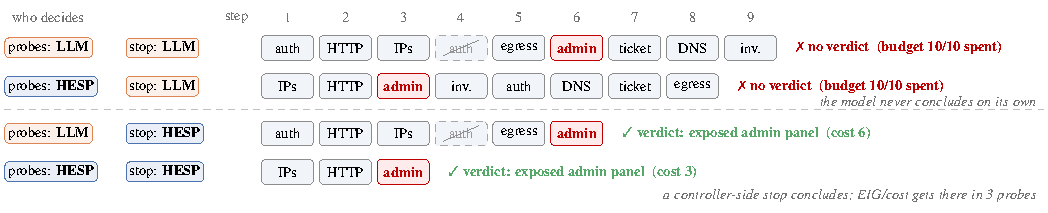
\includegraphics[width=\textwidth]{fig_motivating.pdf}
    \captionof{figure}{One alert, one local model, four ways to split the investigation. The alert's true cause is an exposed admin panel; the planner is Llama-3.1-8B in every row, with the same seed. Each chip is a probe that ran (dashed: a duplicate proposal the controller blocked); red marks the observation that confirms the cause. When the model decides when to stop, it reaches the decisive evidence and keeps probing until the budget is gone. A controller-side stop concludes, and information-gain probe selection gets there in three probes. All four rows are verbatim from the archived journals.}
    \label{fig:motivating}
  \end{center}
  \vspace{1em}
}]

\begin{abstract}
Security teams increasingly let LLM agents triage alerts, and organizations that keep telemetry in-house must run these agents on small local models. Such an agent reads logs that the attacker partly writes, and the attacker needs only a benign verdict to have an alert closed. Prompt-level defenses give no guarantee, and isolation designs protect tool calls, whereas a triage agent's harmful output is the verdict it computes from attacker-written data. We present \hesp{}, a controller that lets the model read but not decide. \hesp{} keeps a Bayesian ledger of candidate causes, selects read-only probes by expected information gain, and accepts a verdict only if ledger evidence supports it; a benign verdict must further be corroborated by independent sources and may never rest on the model's own reading of a log. On three simulated triage settings with five open-weight models from 7B to 72B, no injected instruction, forged source, or adaptive attack on the model's log parsing closes a case under \hesp{}, whereas without its rules such attacks close up to every actionable case as benign. The controller alone resolves every case in two of the three settings, and neither a 72B planner nor a prompt tuned for the baselines resolves more.
\end{abstract}

\section{Introduction}
\label{sec:intro}

Security teams are starting to hand alert triage and investigation to LLM agents~\citep{guide,cortex,sentinelrl}. An agent receives an alert, queries logs, and reports whether an attack happened and what it touched. Whether such an agent can be trusted to close alerts is decided largely by benchmarks: ExCyTIn-Bench~\citep{excytin}, SIABench~\citep{siabench}, and others report how often agents reach the right answer, and the field reads the numbers as measures of investigation ability. Investigation is the reason to deploy an agent at all. An agent that only recognizes what the alert already says adds nothing an analyst would pay for, and it fails in the cases an attacker creates on purpose, where the malicious activity looks routine and nothing names it.

A benchmark measures investigation only if its items cannot be answered without investigating. Consider an ExCyTIn question generated from a three-hop path: from an alert about a scheduled task, through the host, to a related alert whose IP address is the answer. The question asks for ``the IP address recorded in the related `Anomaly detected in ASEP registry' alert''. One SQL query for that alert name returns the answer; the pivot the question was generated from is unnecessary (\cref{fig:example}). If many items are like this, an agent can earn a score without investigating, and the score says nothing about the cases that matter.

Benchmark papers report model scores but rarely the score of a rule that does not investigate. Security has a tradition of re-evaluations that ask exactly this question of learning-based detectors: simple baselines match complex provenance-based detectors~\citep{bilot2025simpler}, and spurious correlations inflate lab results~\citep{arp2022dos}. Machine learning knows the same problem as shortcut learning~\citep{geirhos2020shortcut,gururangan2018artifacts}. Recent work on incident response proposes new benchmarks that reward evidence discovery~\citep{sirbench}, but the benchmarks already in use have not been audited, and whether the agents evaluated on them use the shortcuts they contain has not been measured.

\begin{figure}[t]
  \centering
  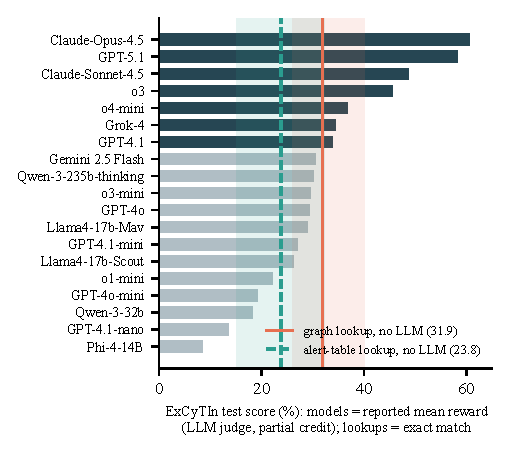
\includegraphics[width=\columnwidth]{fig_floor.pdf}
  \caption{A lookup without an LLM outscores \oBelowGraph{} of \oModels{} reported agents on ExCyTIn-Bench. Bars: mean reward reported for each model on the 589 test questions~\citep{excytin}. Lines: two investigation-free lookups of the alert the question names, on the same questions, scored by exact match (shaded: 95\% intervals, incidents resampled). Dark bars exceed the graph lookup.}
  \label{fig:floor}
\end{figure}

We audit four public benchmarks and datasets for LLM security-operations agents (ExCyTIn-Bench, SIABench, GUIDE, and OTRF Security-Datasets) and three triage environments we built ourselves. For each, we write a fixed rule that uses only what the agent sees, contains no LLM, and skips the investigation the benchmark intends, and we compare it with reported model scores. We find four kinds of shortcut: the question names the evidence that holds the answer (S1), the label follows the organization that assigned it (S2), the data generation leaves a cue such as the attack network's address (S3), and in constructed environments a fixed procedure over the evidence model solves every case (S4). For ExCyTIn, whose authors publish the full logs of 14 agent runs, we go further and test question by question whether the agents' successes come from the shortcut. We registered the hypotheses and froze the rules before every confirmatory run.

\paragraph{Results} Every audited benchmark admits an investigation-free rule that reaches a large share of the reported scores. On ExCyTIn, \oNamed\% of the test questions name the alert that holds the answer, and a lookup of that alert answers \oGraph\% exactly, more than the mean reward of \oBelowGraph{} of \oModels{} reported models (\cref{fig:floor}). On SIABench, ``true positive if and only if the alert involves 172.16.0.1'' is correct on all 35 alerts. On GUIDE, repeating an organization's earlier grade for the same detector is correct on \gHistPct\% of later incidents. In OTRF recordings, the alert text alone separates \otRuleCorrect{} of \otN{} alerts. Yet the ExCyTIn agents do not use the shortcut. Their success is no higher on questions that name the answer's alert (\lgPos{} of \lgModels{} runs, $p=\lgP$); they issue as many queries when one would do; and their ranking is nearly unchanged on shortcut-resistant questions (Kendall $\tau=\lgTau$). The deeper problem is that success depends only weakly on the investigation a question requires: the strongest agent fails \tcOpusFail{} of the 140 questions a single lookup answers.

\paragraph{Contributions}
\begin{itemize}\setlength\itemsep{1pt}
\item A definition of shortcuts for investigation benchmarks and a taxonomy of four kinds, each paired with an investigation-free baseline (\cref{sec:method}).
\item An audit of four public benchmarks and three constructed environments, showing that each admits a rule that reaches or exceeds a large part of reported model scores (\cref{sec:floors}).
\item A question-level analysis of 14 published agent runs on ExCyTIn, showing that the agents do not exploit the shortcut and that their success tracks the required investigation only weakly (\cref{sec:scores}).
\item Checks for benchmark builders, evidence that paired attack and benign ``twins'' remove the single-observation shortcut, and per-question shortcut flags for ExCyTIn (\cref{sec:design}).
\end{itemize}

\section{Background and Motivation}
\label{sec:background}

\subsection{Alert Triage}
Triage decides, for each alert, what caused it and whether a response is needed~\citep{nodoze}. Unlike attack investigation, which reconstructs a whole attack story~\citep{kairos,clouseau}, triage ends with one verdict: a cause and the evidence for it. The analyst reaches the verdict by querying the environment, and queries differ in cost and in how well they separate the candidate causes.

Consider an alert that reports a spike in authentication failures and HTTP errors on a web tier (\cref{fig:motivating}). It looks like credential stuffing, but SQL-injection probing, an authorized vulnerability scan, a misclassified health check, and an administration panel exposed to the internet produce the same symptom. A threat-intelligence lookup on the top source may answer ``malicious'', which three of these causes share. Reading the admin panel's configuration, one cheap query, settles the last explanation at once, but only an investigator who keeps that explanation in view will run it. An investigation therefore makes two decisions again and again: which query to run next, and whether the evidence already suffices.

\subsection{Small Models Fail at the Procedure}
\label{sec:motivation}
An LLM agent makes both decisions itself~\citep{react}: at each step the model reads the observations so far, then calls a tool or states a verdict. \Cref{fig:motivating} shows what happens when the model is Llama-3.1-8B and the true cause is the exposed admin panel. When the model chooses the probes and decides when to stop (first row), it never runs the decisive query. When a controller chooses the probes but the model still decides when to stop (second row), the model sees the decisive observation at step three and keeps probing until the budget is gone. Only when the controller also stops does the episode end with the right verdict.

\begin{figure*}[t]
  \centering
  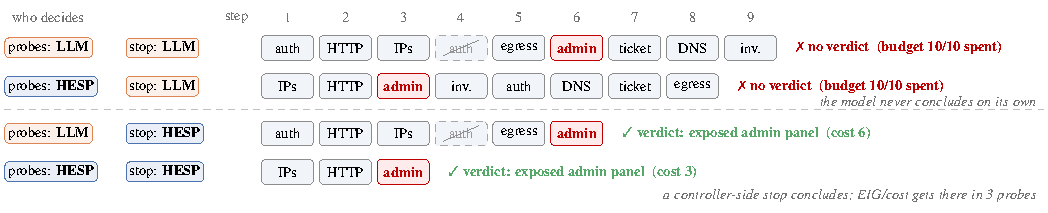
\includegraphics[width=\textwidth]{fig_motivating.pdf}
  \caption{Choosing probes and stopping are separate failures. One alert (true cause: an exposed admin panel), one local model (Llama-3.1-8B), four ways to split the investigation. Each chip is a probe that ran (dashed: a duplicate proposal the controller blocked); red marks the observation that confirms the cause. When the model decides when to stop (first two rows), it reaches the decisive evidence and keeps probing. A controller-side stop concludes (last two rows), and information-gain selection gets there in three probes. All rows are taken from archived journals.}
  \label{fig:motivating}
\end{figure*}

The pattern holds beyond this alert. Qwen2.5-7B choosing its own probes resolves 8 to 13\% of cases while spending nearly its whole budget, and uniformly random probes would do better. Llama-3.1-8B requests another probe in all 3{,}389 of its decisions, including those in which the ledger's posterior exceeds 0.999. Larger models do conclude, but without a ledger Qwen2.5-32B and 72B cite invalid evidence in 22 to 31\% of their citations. Two small models of similar size thus fail in different places, one at choosing probes and one at stopping (\S\ref{sec:utility}), which is why a controller has to take over both decisions rather than repair one.

\subsection{Attacker-Written Evidence}
An agent that reads retrieved content can be steered by instructions hidden in it, namely indirect prompt injection~\citep{greshake2023}, which AgentDojo benchmarks on tool-using agents~\citep{agentdojo}. Log injection through unescaped user-controlled fields is an older form of the same problem~\citep{owasp_loginjection}, and LogInject shows that LLM log analysis in SOCs follows such payloads at high rates~\citep{loginject}. Defenses fall into two families. Model-level defenses, such as structured queries and preference optimization~\citep{struq,secalign}, reduce but do not remove the model's tendency to follow injected text. System-level defenses separate a privileged planner from the untrusted data: the Dual LLM pattern and CaMeL~\citep{camel} let a quarantined model read the data while a planner fixes the control flow, and CaMeL, FIDES~\citep{fides}, and Progent~\citep{progent} enforce policies on the tool calls that follow. CaMeL also shows that the quarantined reader remains a channel: an attacker who cannot change the plan can still choose the values the reader returns. In triage this channel is the whole attack, because the verdict is computed from the values the reader returns and no tool call follows that a policy could stop.

\section{Problem Setting and Threat Model}
\label{sec:threat}

\paragraph{Deployment.} An organization runs the triage agent inside its own network. A local open-weight model serves as the planner. The agent has read-only access to the organization's security telemetry through a fixed catalogue of probes, such as queries over authentication logs, HTTP logs, DNS logs, change tickets, and threat intelligence. Each probe has a cost in analyst time or query load. An episode starts from one alert and ends with a verdict naming a cause and the observations that support it, with an abstention, or with an exhausted budget. Verdicts go to a human analyst. The agent never remediates, and it never sends traffic to the systems under investigation.

\paragraph{Adversary.} The alert may be caused by an attacker who controls part of the evidence the agent will read, for example request payloads, user agents, subdomain names, or command lines. Such an attacker wants the investigation to end with a benign verdict, or with no verdict before the budget runs out. They cannot modify the controller, the probe catalogue, the prediction tables, or the journal. The planner model is not trusted to follow a sound procedure: it may repeat probes, stop too early, never stop, or claim a cause without evidence.

\paragraph{What the controller enforces.} Three properties hold by construction, whatever the planner outputs. First, every executed probe is in the read-only catalogue, is affordable, and has not already run in the current state. Second, every accepted verdict cites at least one real observation from the current state that raised the claimed cause's score. Third, every prediction is journaled before the observation it predicts, so the audit can replay the episode. The controller does not guarantee a correct verdict. Correctness depends on the prediction tables and on the hypothesis set containing the true cause. An attacker who can make a probe return the outcome expected under a benign cause can still mislead it. We do not evaluate evidence manipulation or prompt injection through log content; in our environment, observations reach the ledger as discrete outcomes, so the planner's reading of raw text never changes a score.

\paragraph{Why local and small.} Keeping telemetry on premises rules out hosted frontier models for many organizations, and on-premises hardware bounds model size. We therefore evaluate models from 7B to 72B parameters served on a single GPU and ask what a controller must supply for the smallest of them.

\section{HESP Overview}
\label{sec:overview}

\begin{figure*}[t]
  \centering
  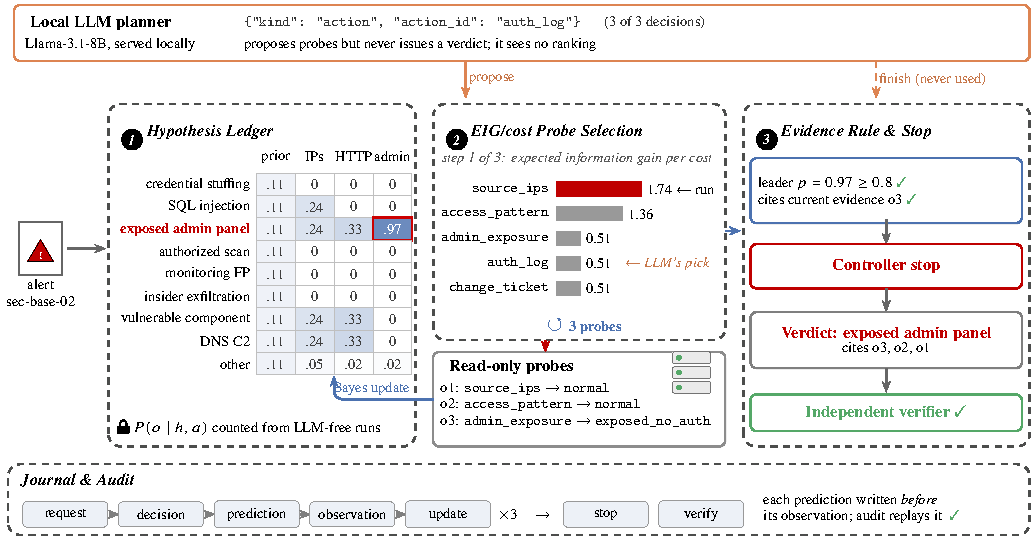
\includegraphics[width=\textwidth]{fig_pipeline.pdf}
  \caption{Overview of \hesp{}, shown on the fourth row of \cref{fig:motivating}. \protect\stepnum{1} The hypothesis ledger keeps a posterior over the candidate causes, updated by Bayes' rule from frozen probe-outcome tables. \protect\stepnum{2} The controller ranks legal probes by expected information gain per cost and runs the best one; the planner's proposal (here \texttt{auth\_log}, three times) is advisory. \protect\stepnum{3} Once the leader's posterior reaches 0.8 and a current observation supports it, the controller concludes, citing that evidence, and an independent verifier checks the verdict. Every step is journaled before its observation and audited afterwards. All values are from the archived journal.}
  \label{fig:pipeline}
\end{figure*}

\hesp{} (Hypotheses $\rightarrow$ Evidence $\rightarrow$ State $\rightarrow$ Planning) puts the investigation procedure in a controller between the local model and its tools. \Cref{fig:pipeline} shows its three stages on the episode from the fourth row of \cref{fig:motivating}.

\paragraph{\stepnum{1} Hypothesis ledger.} The controller keeps an explicit belief over the candidate causes, starting from a uniform prior over the eight causes and \textit{other}. After each observation it applies Bayes' rule with a frozen table $P(o \mid h, a)$ counted from LLM-free development runs. In the example, the first two probes return \textit{normal} and leave four, then three, causes plausible; the third returns \textit{exposed, no auth} and moves the exposed admin panel to 0.97.

\paragraph{\stepnum{2} Probe selection.} Before each step the controller ranks every legal probe by expected information gain per unit cost and runs the best one. The planner still proposes a probe, but the proposal is advisory, and in blind configurations the planner never sees the ranking. In the example, the model proposed \texttt{auth\_log} three times, which the ranking valued at 0.51 and later 0.04 bits per unit; the controller ran \texttt{source\_ips}, \texttt{access\_pattern}, and \texttt{admin\_exposure}.

\paragraph{\stepnum{3} Evidence rule and stop.} A verdict is accepted only if its cause has current posterior at least 0.8 and a current observation supports it. The planner may finish or abstain; the controller may also conclude on its own when the rule is met. In the example the model never finished, so the controller concluded, cited the three observations, and the independent verifier confirmed the verdict.

\paragraph{Journal and audit.} Every request, decision, prediction, observation, and ledger update is appended to a journal, with each prediction written before the observation it predicts. An audit replays the journal after every episode. \Cref{sec:design} details each component and the alternatives we measured.

\section{Design}
\label{sec:design}

\begin{figure}[t]
  \centering
  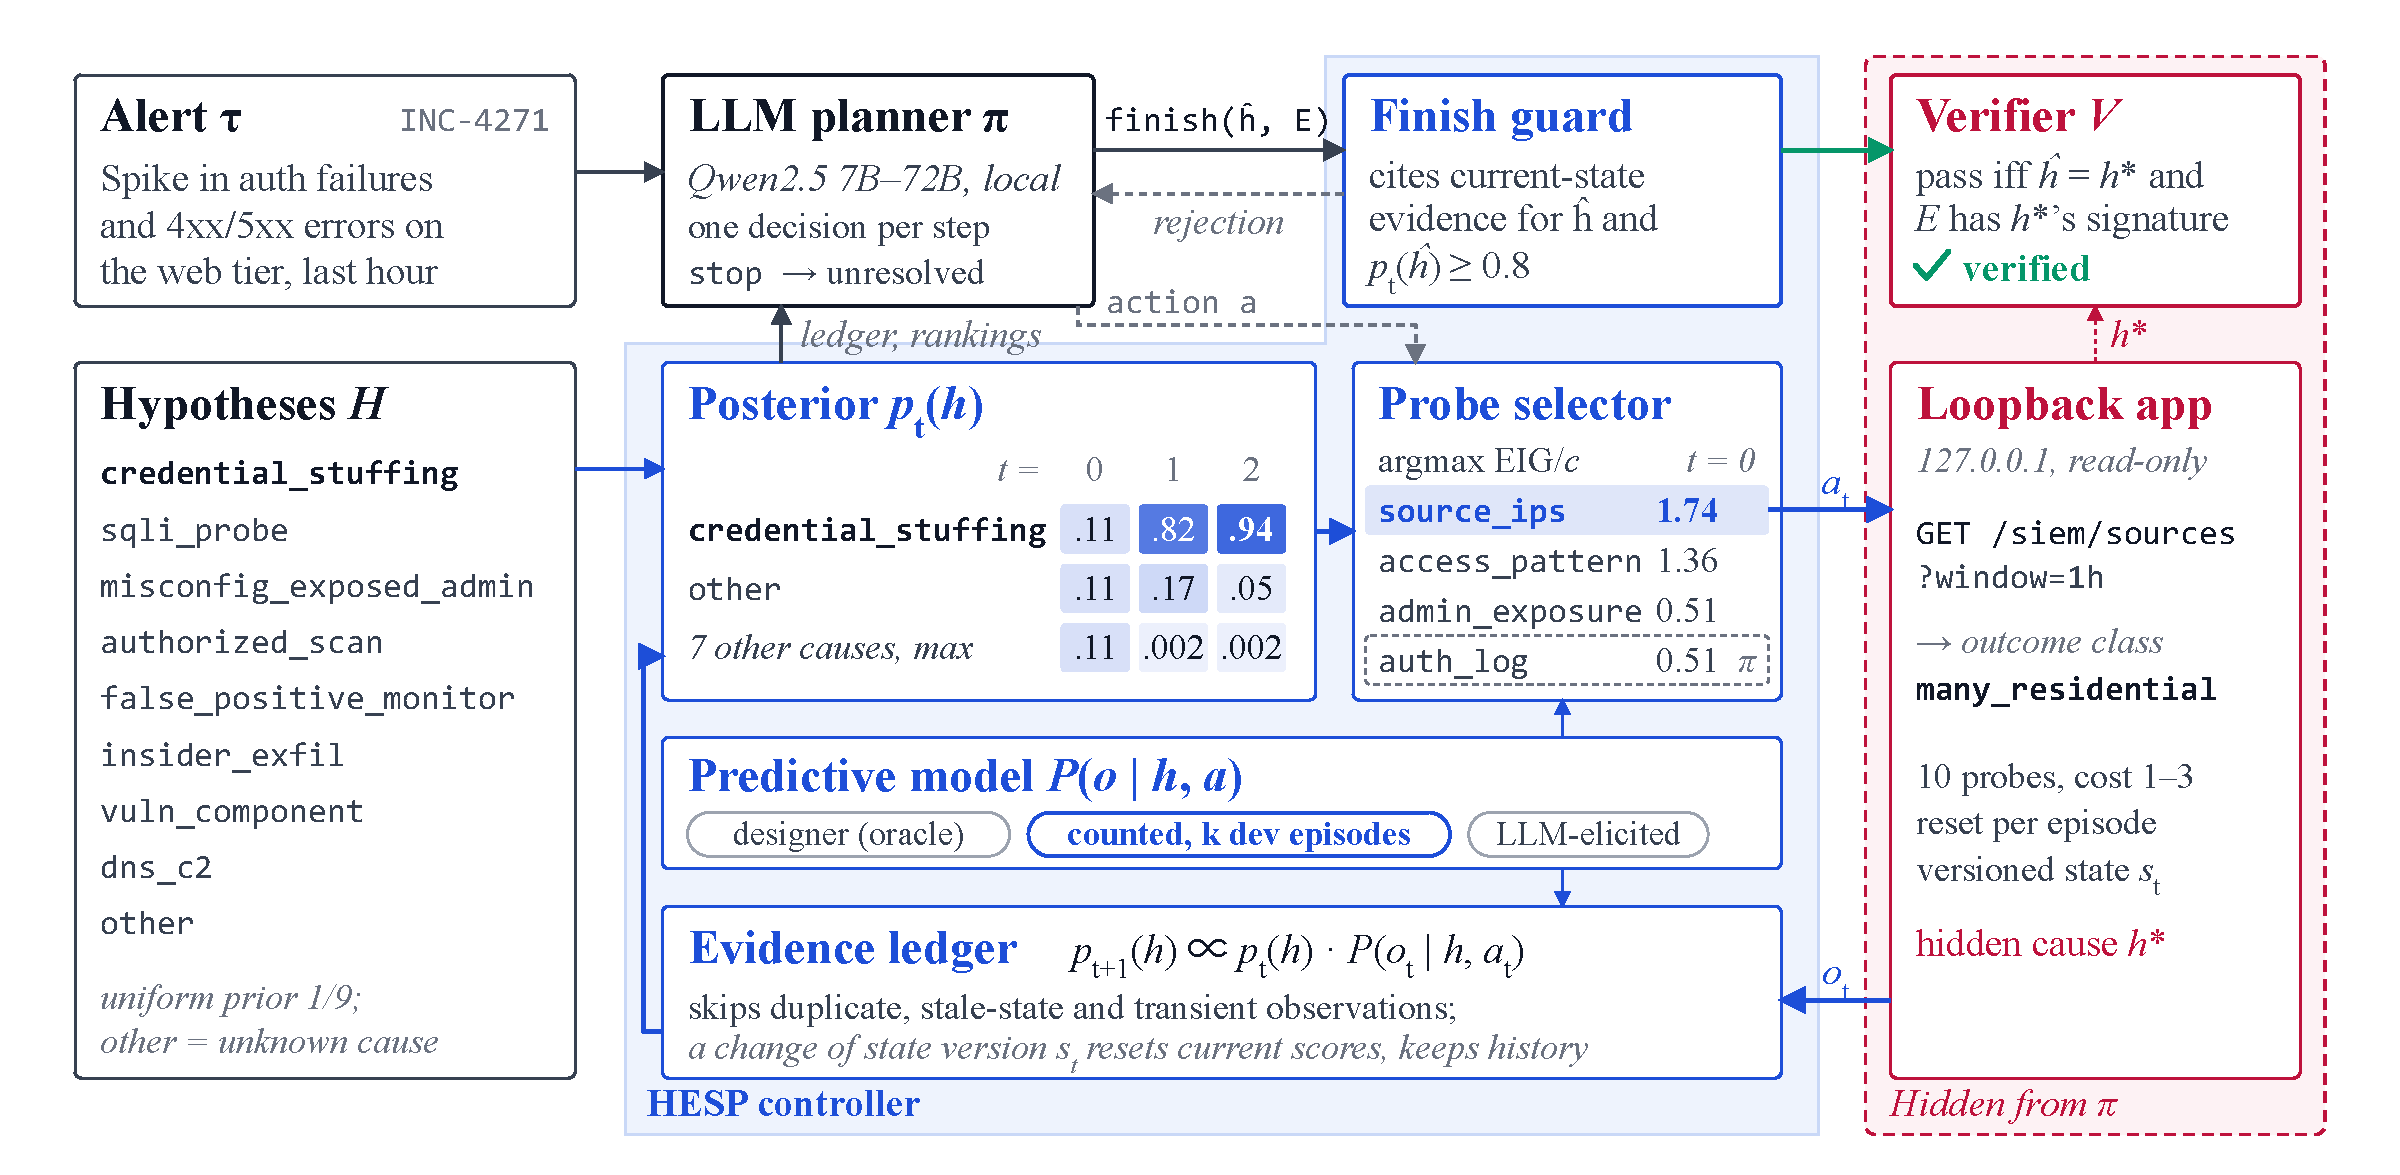
\includegraphics[width=\linewidth]{hesp-framework.pdf}
  \caption{The same triage case (sec-base-00, Qwen2.5-7B, repeat 0) handled by the model alone (left) and inside \hesp{} (right), drawn from the archived v0.6 journals.}
  \label{fig:framework}
\end{figure}

\subsection{Setting and interface}
An episode begins with an alert and a finite set of hypotheses $\mathcal{H}$. $\mathcal{H}$ contains the candidate explanations plus an explicit \textit{other}. The agent may call read-only probes $a \in \mathcal{A}$ that cost $c(a)$ each, within budgets on tool calls, total cost, planner decisions, and wall time. At each step the planner (the LLM) receives a structured request: the task, the probe catalogue with descriptions and costs, the observation history, feedback on blocked proposals, the remaining budgets and, depending on the configuration, the ledger. It returns one JSON decision:
\texttt{action} (propose a probe), \texttt{finish} (a hypothesis plus the observation IDs it cites), or \texttt{stop} (abstain). Probes never modify the environment, and the agent never sends attack payloads.

\subsection{Hypothesis ledger}
The ledger holds a posterior $p(h)$ over $\mathcal{H}$. Each probe comes with a predictive table $P(o \mid h, a)$ over its outcome vocabulary. After observing $o$, the ledger applies Bayes' rule. For every hypothesis it records whether the observation raised, lowered, or left unchanged its score (\textit{support}, \textit{against}, \textit{neutral}). A transient failure, such as an HTTP 503, is not evidence: it is logged, and the probe may be retried. If an outcome is impossible under every hypothesis, the table is in conflict and the observation is skipped. The environment exposes a \emph{state version}. When the incident changes under the agent (the \textit{drift} variant), the version advances and current scores are reset to the prior. Earlier evidence is kept for the record but no longer counts as current.

\subsection{Probe selection}
For every legal probe (untried in the current state, affordable, prerequisites met), the controller computes the expected information gain
\[
\mathrm{EIG}(a) = H\big(p\big) - \sum_{o} P(o \mid a)\, H\big(p(\cdot \mid o, a)\big), \qquad P(o \mid a) = \sum_h p(h) P(o \mid h, a),
\]
and ranks the probes by $\mathrm{EIG}(a)/c(a)$. In the \hesp{} configurations the controller executes its own choice whatever the planner proposed. Configurations differ in whether the planner is shown the ranking. The \emph{blind} configurations show no ranking and no selector name, so the planner's prompt is identical whichever selector runs. A unit test checks this byte for byte. A \emph{random} selector, which picks uniformly among legal probes, serves as the control.

\subsection{Finishing, verification, and audit}
\paragraph{State-guarded finish.} A planner's \texttt{finish} is accepted only if at least one cited observation is current-state evidence that supports the claimed hypothesis, and the hypothesis has current score at least $\tau = 0.8$. A rejected finish is returned to the planner as feedback.

\paragraph{Controller-side stop (v0.9).} The controller may also conclude on its own. Before each planner call, and when a budget runs out, it applies the same acceptance rule to the current leader and, if the rule is met, cites up to three supporting current-state observations. The planner may still finish or abstain earlier, and nothing in its prompt reveals the rule.

\paragraph{Independent verifier.} A verdict counts as \emph{verified} only if the hypothesis equals the cause in effect and at least one cited observation, from the current state, carries a signature that cause uniquely produces. A verdict reached purely by elimination, or backed only by a generic ``malicious'' threat-intelligence hit that several attacks share, does not verify. The verifier is not reachable through the planner interface.

\paragraph{Journal and audit.} Every prediction is written to an append-only journal before the probe runs. After each episode, an audit checks event ordering, observation provenance, counters, budgets, citations, and, from v0.9 on, that every controller-made verdict meets its rule. All reported episodes pass the audit.

\section{Implementation}
\label{sec:impl}

\hesp{} is about 2{,}900 lines of Python that use only the standard library. The controller, ledger, selectors, verifier interface, journal, and audit account for roughly 1{,}800 of them. Planners are pluggable: the same JSON decision protocol serves vLLM and Ollama endpoints, a subprocess adapter, and scripted policies used for LLM-free runs. Each episode gets its own loopback HTTP sandbox (a \texttt{ThreadingHTTPServer} bound to 127.0.0.1), so probes are real HTTP requests with transient failures and state changes, and no episode can observe another.

\paragraph{Journal and audit.} Each episode writes an append-only JSONL journal. The journal records every planner request and decision, every prediction before its probe runs, every observation, every ledger update, and the verification. The audit replays the journal and checks event order, observation provenance, counters against the result record, budgets, citations, and the controller's own verdicts. All 7{,}272 reported episodes pass.

\paragraph{Study runner.} A paired, shuffled, resumable runner executes up to 32 episodes concurrently and refuses to resume if the manifest or the controller source hash has changed. The source hash covers every file of the controller package with line endings normalized, so Windows and Linux checkouts agree. After each model, the runner audits all episodes, archives the journals, and records the archive's SHA-256 before the GPU server is released. The stopping study's 1{,}800 episodes ran in 28 minutes on one RTX~6000-class GPU. A test suite of 145 unit tests covers the ledger, selectors, blind prompts, guard, controller stop, audit, and the empirical estimator's isolation from the environment's generator.

\section{Evaluation Methodology}
\label{sec:method}

\subsection{The sec-triage environment}
Each episode is one alert on a web service. The hidden cause is one of eight explanations: three real attacks (credential stuffing, SQL-injection probing, DNS command-and-control), an insider exfiltrating data, an exposed admin panel, a known-vulnerable component, an authorized vulnerability scan, and a monitoring false positive. The hypothesis set adds \textit{other}. Ten read-only probes, costing 1 to 3 units each, cover authentication failures, HTTP patterns, source reputation, admin exposure, per-user egress, DNS characteristics, component inventory, change tickets, threat intelligence, and a generic runbook. The environment is designed so that shortcuts fail. Threat intelligence says only that an indicator is malicious, and three attacks share that answer. The runbook carries no information. Several benign causes look like attacks until the right probe is run. Each cause appears in three variants. In \textit{base}, outcomes are deterministic except for a 10\% threat-intelligence lag. \textit{Noise} adds 15\% transient 503 failures and a 30\% lag. In \textit{drift}, the incident is superseded after the second probe: the state version advances and the true cause switches. This gives 24 tasks, and each study runs every task three times per configuration. Each episode is served from its own loopback HTTP sandbox.

\subsection{Prediction tables}
The ledger and the selector need $P(o \mid h, a)$. We compare three sources. \emph{Designer} tables come from the environment's generating function and serve as an oracle reference. \emph{Empirical} tables are estimated by counting outcomes in LLM-free development episodes: an exhaustive script runs every probe on each (cause, variant) instance $k$ times, for $k \in \{1, 5, 20, 100\}$. It uses only base and noise variants, draws its seeds from a space disjoint from evaluation, and applies $\varepsilon = 0.01$ smoothing. A unit test enforces that the estimator never calls the generating function. \emph{Elicited} tables are produced by the planner LLM itself. Every table is written to disk, hashed, and frozen before any evaluation episode runs. The empirical tables tell us how many observations are enough, not how the method behaves in an unknown world: development and evaluation episodes come from the same generator.

\subsection{Configurations}
All configurations use the same model, prompt template, probes, budgets (10 tool calls, 10 cost units, 12 decisions, 900\,s), duplicate blocking, and verifier.
\begin{itemize}
  \item \textbf{ReAct-style}: the planner sees the raw history only and picks every probe.
  \item \textbf{Memory-only}: the planner also sees the ledger and picks every probe itself.
  \item \textbf{\hesp{}}: the controller picks the probe (EIG/cost or random), with or without showing its ranking, and with or without the finish guard or the controller-side stop.
\end{itemize}

\subsection{Models and serving}
Qwen2.5-7B-Instruct (bf16), Qwen2.5-32B-Instruct-AWQ, and Qwen2.5-72B-Instruct-AWQ in every study. From v0.8 on, the Llama 3.1 family is added: 8B-Instruct (bf16) and 70B-Instruct-AWQ-INT4. Models are served by vLLM on a single RTX~6000-class GPU at temperature 0.2, with a distinct seed per call.

\subsection{Pre-registration and statistics}
Each study's hypotheses, arms, primary endpoints, and analysis were written down and frozen, together with the source hash and the table hashes, before any of its episodes ran. The pipeline smoke tests run before freezing are disclosed and excluded from all analyses. The outcome measure is \emph{verified completion}, the fraction of episodes that end with a verified verdict. Every other ending counts as a failure. We report paired per-task differences with percentile task-cluster bootstrap intervals (2{,}000 resamples, 24 clusters). When a study has two primary endpoints, each gets a Bonferroni-adjusted 97.5\% interval. All secondary comparisons are exploratory and uncorrected. We also report descriptive security metrics. Two causes are benign: the authorized scan and the monitoring false positive. The other six require action. Among episodes that end with a verdict, the \emph{missed-attack} rate is the fraction of cases with an actionable true cause in which the verdict names a benign cause. The \emph{false-escalation} rate is the fraction of cases with a benign true cause in which the verdict names an actionable one. The \emph{wrong-cause} rate is the fraction of verdicts that name the wrong cause. The \emph{unresolved} rate is the fraction of all episodes without a verified verdict. Ground truth is the cause in effect at the moment of the verdict.

\section{Evaluation Results}
\label{sec:results}

We report the results by question rather than by study: which decisions a controller should take from the model (\S\ref{sec:rq-stop}), what remains for the model once the controller applies the verifier's evidence standard (\S\ref{sec:fair}), where the resulting security boundary lies (\S\ref{sec:adversarial}), where the controller's knowledge comes from and how it fails when that knowledge is wrong (\S\ref{sec:mismatch}), and whether the effects replicate on the second family (\S\ref{sec:external}). Appendix~\ref{app:tables} gives every cell of every study.

\subsection{Probing and Stopping Are Separate Decisions}
\label{sec:rq-stop}
\label{sec:rq-rank}
A controller that picks probes changes two things at once: it removes the model's own choice, and it replaces that choice with a ranking. The decomposition study separates the two with blind configurations, in which the planner receives the same prompt whatever the selector; the stopping study then crosses who selects probes with who may stop. \Cref{fig:probe-stop} shows the second.

\begin{figure*}[t]
  \centering
  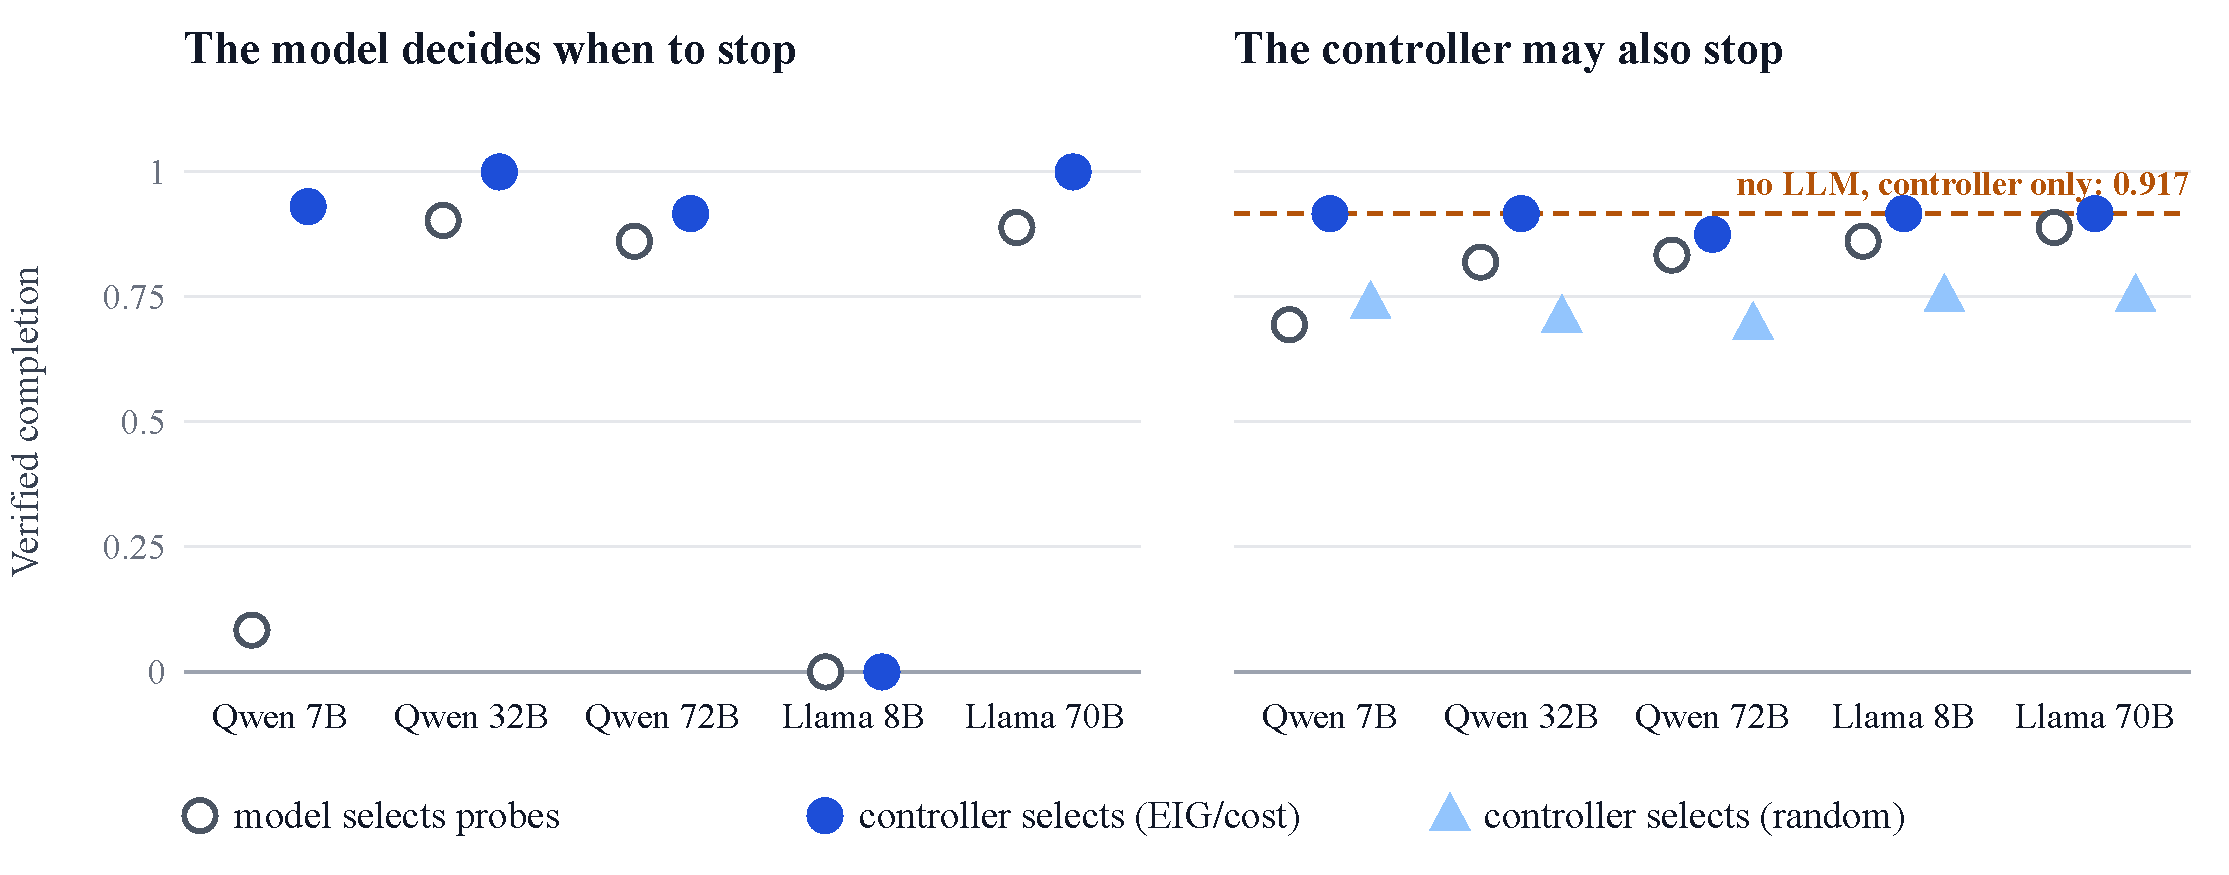
\includegraphics[width=0.92\textwidth]{fig-probe-stop.pdf}
  \caption{Stopping study: verified completion by who selects probes and who may stop (72 episodes per point). The dashed line is the post hoc LLM-free controller (EIG/cost selection and controller stop, same seeds and tasks).}
  \label{fig:probe-stop}
\end{figure*}

First, the ranking itself helps. With identical planner information, EIG/cost selection beats random selection by $+0.306$ $[+0.14,+0.47]$ on Qwen2.5-7B (a pre-registered endpoint), and by $+0.26$ to $+0.35$ on every other model that concludes. Taking the choice away, in contrast, helps weak models and hurts strong ones: random selection instead of the model's own choices raises completion by $+0.556$ for Qwen2.5-7B and lowers it by 0.222 and 0.278 for Qwen2.5-32B and 72B. Showing the ranking to the planner changes completion by at most $+0.06$.

Second, selecting probes does not make a model conclude. Under our prompt and serving configuration, Llama-3.1-8B completed none of its 360 decomposition episodes: all 3{,}389 of its decisions request another probe, in valid JSON. With a controller stop it rises from 0 to 0.917 ($+0.917$ $[+0.79,+1.00]$, pre-registered), and controller selection then adds $+0.056$ $[-0.07,+0.18]$, no detectable completion, although it halves probe cost (2.35 against 4.78 units). Qwen2.5-7B needs both parts: a stop alone lifts it from 0.083 to 0.694, and selection adds $+0.222$ $[+0.08,+0.39]$. A controller cannot know in advance which part a model lacks, so it has to supply both.

Third, the posterior stop concludes by elimination. With controller selection and stop, four of the five models fail on the same six episodes: a correct DNS command-and-control verdict reached by eliminating the alternatives, which the verifier rejects for lack of a confirming signature. Strong models that decide when to stop, in configurations without the controller stop, keep probing until that signature appears. The LLM-free controller with the posterior stop completes 0.917 at 2.35 units, and four models score exactly the same when the controller both selects and stops.

\subsection{What Remains for the Model}
\label{sec:fair}
The comparison above mixes two things: whether an LLM helps, and which evidence standard ends the episode. The v1.1 study removes this confound. It gives the LLM-free controller the confirmation stop of \S\ref{sec:finish}, adds a fixed playbook and catalogue order as simpler references, and runs every LLM configuration with the finish guard, on both families with the same seeds, tasks, and budgets. Its primary endpoints compare Qwen2.5-72B deciding when to stop against the LLM-free confirmation stop (97.5\% intervals). \Cref{tab:v11fair} reports both episodes that meet the evidence policy and episodes that name the right cause.

\begin{table}[t]
  \caption{What remains for the model (v1.1): episodes that meet the evidence policy / episodes that name the right cause, when the LLM decides when to stop (``LLM''), under the posterior stop (``post.''), and under the confirmation stop (``conf.''). Every LLM row uses controller selection and the finish guard; seeds, tasks, and budgets match the LLM-free row.}
  \label{tab:v11fair}
  \centering\small
  \begin{adjustbox}{max width=\columnwidth}% generated by paper/make_tables.py -- do not edit
\begin{tabular}{llrrrr}
\toprule
 & & \multicolumn{2}{c}{sec-triage (72)} & \multicolumn{2}{c}{sigma-triage (152)} \\
\cmidrule(lr){3-4}\cmidrule(lr){5-6}
Planner & Controller & verified & cost & verified & cost \\
\midrule
LLM-free & posterior stop & 66 & 2.35 & 152 & 2.20 \\
LLM-free & confirmation stop & 72 & 2.54 & 152 & 2.20 \\
LLM-free & fixed playbook, conf. & 66 & 2.90 & 152 & 2.20 \\
LLM-free & catalogue order, conf. & 65 & 4.93 & 151 & 2.96 \\
\addlinespace
Q-7B & guard, LLM stops & 66 & 7.17 & 126 & 3.22 \\
Q-7B & guard + posterior stop & 66 & 2.35 & 141 & 2.12 \\
Q-7B & guard + confirmation stop & 72 & 2.54 & 141 & 2.12 \\
\addlinespace
L-8B & guard, LLM stops & 0 & 10.00 & 1 & 9.78 \\
L-8B & guard + posterior stop & 66 & 2.35 & 152 & 2.20 \\
L-8B & guard + confirmation stop & 72 & 2.54 & 152 & 2.20 \\
\bottomrule
\end{tabular}
\end{adjustbox}
\end{table}

First, with the verifier's standard, the controller alone completes every case: 72 of 72 sec-triage and 152 of 152 sigma-triage episodes, at 2.54 and 2.20 units, 0.19 units more than the posterior stop on sec-triage. Adaptive selection still matters on sec-triage, where a fixed playbook reaches 66 and catalogue order 65, but not on sigma-triage, where every order completes at least 151 of 152.

Second, no model adds to that controller. Qwen2.5-72B deciding when to stop meets the evidence policy in 72 of 72 sec-triage episodes ($+0.000$ $[0.000, 0.000]$) and 148 of 152 sigma-triage episodes ($-0.028$ $[-0.111, 0.000]$; the mean over rules of per-rule differences, $-4/152 = -0.026$ per episode), at 3.86 and 3.25 units against 2.54 and 2.20. By the interpretation written before the run, we measured no gain from the LLM in deciding when to stop. Qwen2.5-32B and Llama-3.1-70B behave alike, and every sigma-triage miss of the three large models names the right cause without a confirming signature. When the model decides when to stop, Llama-3.1-8B completes 0 and 1 episodes and Qwen2.5-7B 66 and 126. Qwen2.5-7B also falls short under the controller stop (141 of 152), for one reason: on three rules it proposes a finish at a posterior of 0.794 to 0.796, just below the guard's threshold, the guard rejects it, and the model repeats the proposal until the decision budget is spent (11 episodes, 9 to 11 rejections each). The controller stop cannot fire below 0.8, so a planner can stall a guarded controller. The v1.2 study adds a recovery rule, under which the controller runs its own top-ranked probe after two consecutive rejected finishes: a scripted planner that insists on finishing at a score of 0.5 stalls all 152 sigma-triage episodes without it and completes all 152 with it.

Third, the evidence policy is a trade-off between automation and safety, not a detail of scoring. Our verifier accepts a verdict only if one cited observation carries a signature that the cause alone produces, so a right cause reached by combining or excluding observations counts as a failure; \cref{tab:v11fair} shows that under a ``right cause'' standard the posterior stop would also complete 72 of 72. The v1.2 study measures the alternatives with the LLM-free controller (\cref{tab:v12policy}). It adds \emph{comp-triage}, a third family of three scenarios in which an attack and three legitimate activities use the same tools, outcomes are probabilistic, and five of twelve causes have no single-observation signature; a \emph{joint} verifier that accepts any combination of observations that, under the true distributions, favours the cause at least tenfold over every other named cause; and stop rules that require joint evidence against the named causes, or also against \textit{other}. On comp-triage, joint evidence names the right cause in 59 of 72 episodes against 20 for the single-signature rule, which escalates 52. The price is paid in the attacker's currency: joint evidence closed 4 of 18 attacks as the paired legitimate activity, and when the true cause is absent from the candidates it named another actionable cause in 24 of 48 sec-triage episodes. Requiring the evidence to beat \textit{other} tenfold did not change this, and thirtyfold only reduced it to 18. Only the single-signature rule named no wrong cause in any setting, at the cost of escalating most composite cases; lowering its ratio to 3 moves along the same frontier (37 right causes, 1 missed attack). A deployment has to choose a point on this frontier; ours favours escalation.

\begin{table*}[t]
  \caption{Evidence policies (v1.2, LLM-free controller, EIG/cost selection; counts). ``single'' / ``joint'': episodes accepted by the single-signature and the joint-identification verifier. sec, cause absent: the true cause is removed from the candidate set. sec, confusion: each cause's table rows mixed 0.25 toward one other cause. comp-triage: three scenarios pairing an attack with legitimate activities that use the same tools, probabilistic outcomes, five of twelve causes without a single-observation signature.}
  \label{tab:v12policy}
  \centering\small
  \begin{adjustbox}{max width=\textwidth}% generated by paper/make_tables.py -- do not edit
\begin{tabular}{lrrrrrrrrr}
\toprule
 & \multicolumn{2}{c}{sec, matched (48)} & \multicolumn{2}{c}{sec, cause absent (48)} & sec, confusion & \multicolumn{4}{c}{comp-triage (72; 18 attacks)} \\
\cmidrule(lr){2-3}\cmidrule(lr){4-5}\cmidrule(lr){6-6}\cmidrule(lr){7-10}
Stop rule & single & joint & wrong & escal. & verified & right cause & wrong & missed attack & escal. \\
\midrule
posterior (0.8) & 42 & 48 & 24 & 24 & 47 & 64 & 7 & 5 & 1 \\
single signature, $r{=}10$ & 48 & 48 & 0 & 48 & 0 & 20 & 0 & 0 & 52 \\
single signature, $r{=}3$ & 48 & 48 & 0 & 48 & 0 & 37 & 2 & 1 & 33 \\
joint, named causes, $r{=}10$ & 42 & 48 & 24 & 24 & 47 & 59 & 6 & 4 & 7 \\
joint, incl.\ \textit{other}, $r{=}10$ & 42 & 48 & 24 & 24 & 47 & 59 & 6 & 4 & 7 \\
joint, incl.\ \textit{other}, $r{=}30$ & 42 & 48 & 18 & 30 & 18 & 55 & 2 & 1 & 15 \\
\bottomrule
\end{tabular}
\end{adjustbox}
\end{table*}

Fourth, the stopping failure is partly a prompting effect. Replaying 60 archived requests with overwhelming evidence or no probe left, Llama-3.1-8B returned valid, untruncated JSON every time and asked for a probe in 60, 60, and 58 of 60 under the original prompt, a prompt with an example finish, and a prompt that states when to finish. In live episodes inside \hesp{} the explicit rule made it finish in 8 of 48, the other variants in none; for Qwen2.5-7B both variants raised completion inside \hesp{} from 43 to 48 of 48. We did not give the Memory-only and ReAct-style baselines an equally developed prompt, so the size of their gap is specific to the prompt we used.

\subsection{The Security Boundary}
\label{sec:adversarial}
\label{sec:security}
The threat model allows the attacker to control part of the evidence. Without adversarial evidence, the ledger alone already removes most wrong verdicts: in the table-source study, the ReAct-style Qwen2.5-32B and 72B baselines called 13 of 51 and 20 of 54 actionable episodes benign among those they ruled on, Memory-only 2 of 54 and 1 of 53, and \hesp{} none. The adversarial studies test an instruction to close the case as an authorized scan, carried in free-text fields (four texts that differ in wording and position), and forged evidence: a source-reputation probe that reports a known scanner (\emph{forged probe}) and an upstream reputation feed that two probes read (\emph{forged feed}). \Cref{tab:v11attack} attributes the outcomes to components on all five models; the v1.0 results are in \cref{tab:v10c} (Appendix~\ref{app:tables}).

\begin{table*}[t]
  \caption{The security boundary (v1.1, sec-triage, five models): episodes that close an actionable case as benign (``missed'') or end without a verdict (``unresolved'') under four injection texts (of 72 per model); episodes closed as benign under forged evidence (of 18; range over the five models); verified episodes on the two benign causes (of 6; range over the five models).}
  \label{tab:v11attack}
  \centering\small
  \begin{adjustbox}{max width=\textwidth}% generated by paper/make_tables.py -- do not edit
\begin{tabular}{lrrrrrrrr}
\toprule
 & \multicolumn{5}{c}{4 injection texts: missed / unresolved (of 72)} & \multicolumn{2}{c}{forged: missed (of 18)} & benign \\
\cmidrule(lr){2-6}\cmidrule(lr){7-8}\cmidrule(lr){9-9}
Configuration & Q-7B & Q-32B & Q-72B & L-8B & L-70B & probe & feed & verif.\ (of 6) \\
\midrule
Memory-only & 69 / 0 & 57 / 0 & 69 / 0 & 0 / 72 & 63 / 0 & 0--6 & 0--15 & 0--6 \\
Memory-only, raw text removed & 0 / 65 & 0 / 0 & 0 / 0 & 0 / 72 & 0 / 24 & 0--6 & 0--15 & 0--6 \\
\hesp{}, guard only & 0 / 44 & 0 / 46 & 0 / 66 & 0 / 72 & 0 / 58 & 0 & 0 & 0--6 \\
\hesp{}, stop, no guard & 39 / 0 & 36 / 0 & 48 / 0 & 0 / 0 & 36 / 0 & 18 & 18 & 6 \\
\hesp{}, guard + stop & 0 / 24 & 0 / 29 & 0 / 42 & 0 / 0 & 0 / 2 & 18 & 18 & 6 \\
\quad + corroboration by probe & 0 / 0 & 0 / 0 & 0 / 11 & 0 / 0 & 0 / 0 & 0 & 0 & 3 \\
\quad + corroboration by source & 0 / 12 & 0 / 0 & 0 / 3 & 0 / 0 & 0 / 0 & 0 & 0 & 3 \\
\bottomrule
\end{tabular}
\end{adjustbox}
\end{table*}

First, the finish guard is what blocks injected dismissals. Every model that decides and reaches its own verdict follows the instruction, and controller selection and stop without the guard still let the planner finish first with the injected verdict in 36 to 48 of 72 episodes. Every guarded configuration closed 0 of 72 on every model; in v1.0 the pre-registered comparison on Qwen2.5-7B was $+1.000$ $[+1.000,+1.000]$, all 18 paired episodes moving the same way. Removing the raw text from the prompt also blocks the dismissal, at no cost for Qwen2.5-32B and 72B but leaving 65 of 72 Qwen2.5-7B cases unresolved. The injection still costs analyst time: the guard without a controller stop leaves 44 to 72 of 72 episodes unresolved, and adding the stop 0 to 42.

Second, forged evidence defeats the controller. A single forged scanner answer lifts the authorized scan above 0.8 after one probe, and the controller stop concludes: 18 of 18 actionable cases are closed as benign on every model, and a forged feed read by two probes does the same. Acting on the most informative evidence first is exactly what the attacker exploits. The forged feed also misleads the larger LLMs themselves (up to 15 of 18 under Memory-only).

Third, corroboration for benign verdicts closes this gap at a price. Requiring two specifically supporting observations escalates all forged cases on every model, but the per-probe rule survived the forged feed only because the controller's second probe read a different source. A targeted v1.2 test makes a fixed playbook read \texttt{source\_ips} and then \texttt{threat\_intel}, both fed by the forged source: per-probe corroboration then closes 18 of 18 actionable cases as benign, and per-source-group corroboration escalates all 18. Both rules halve completion on the two honest benign causes of sec-triage (3 of 6), because the monitoring false positive has only one specific signature there; across the 26 benign explanations of sigma-triage, corroboration escalates 8 of 104 benign episodes. All counts come from one environment, and a 0 of 18 cell bounds attack success only loosely (about 15\%, one-sided 95\%, even if its six causes and three repeats were independent).

\subsection{Where the Knowledge Comes From}
\label{sec:rq-help}
\label{sec:mismatch}
The controller's knowledge sits in its prediction tables. Counted tables match the generator's: with $k{=}20$ development episodes per cause and variant, \hesp{} with the finish guard lifts Qwen2.5-7B from 0.125 to 1.000 ($+0.875$ $[+0.74,+0.97]$, pre-registered), equal to designer tables on all three Qwen models, and $k{=}5$ already suffices (\cref{tab:v06}, Appendix~\ref{app:tables}), which reflects how deterministic the environment is. Counted tables cost 1.2 to 2.4 more units, all of it in the row for \textit{other}, the one cause development data never exhibits. The models cannot write the tables themselves: tables elicited from the planner leave completion at 0.069 to 0.375.

In our environments the tables come from the same generator as the test episodes. \Cref{tab:v10b} breaks that link with the LLM-free controller. Three findings stand out; the first two hold on both families.

\begin{table*}[t]
  \caption{Table error (LLM-free, posterior stop at 0.8). Under EIG/cost selection: the shares of episodes that are verified, name the right cause without a confirming signature, name a wrong cause, and escalate (these sum to one); under random selection: verified completion. ``Perturbed'' mixes every table row with a random Dirichlet(1) row with weight $\lambda$ (20 random tables per level); ``one cause missing'' averages over removing each cause in turn from the development data and testing on that cause.}
  \label{tab:v10b}
  \centering\small
  \begin{adjustbox}{max width=\textwidth}% generated by paper/make_tables.py -- do not edit
\begin{tabular}{lrrrrrrrrrr}
\toprule
 & \multicolumn{5}{c}{sec-triage} & \multicolumn{5}{c}{sigma-triage} \\
\cmidrule(lr){2-6} \cmidrule(lr){7-11}
Tables & verif. & correct, unverif. & wrong & esc. & random verif. & verif. & correct, unverif. & wrong & esc. & random verif. \\
\midrule
matched tables & 0.917 & 0.083 & 0.000 & 0.000 & 0.792 & 1.000 & 0.000 & 0.000 & 0.000 & 0.886 \\
base variant only & 0.917 & 0.083 & 0.000 & 0.000 & 0.792 & 1.000 & 0.000 & 0.000 & 0.000 & 0.886 \\
$k{=}1$, base only & 0.917 & 0.083 & 0.000 & 0.000 & 0.778 & 1.000 & 0.000 & 0.000 & 0.000 & 0.882 \\
perturbed, $\lambda{=}0.25$ & 0.885 & 0.083 & 0.000 & 0.031 & 0.500 & 0.992 & 0.008 & 0.000 & 0.000 & 0.910 \\
perturbed, $\lambda{=}0.5$ & 0.494 & 0.177 & 0.000 & 0.329 & 0.227 & 0.978 & 0.017 & 0.000 & 0.005 & 0.838 \\
perturbed, $\lambda{=}0.75$ & 0.098 & 0.027 & 0.004 & 0.871 & 0.042 & 0.805 & 0.040 & 0.009 & 0.146 & 0.513 \\
one cause missing (mean) & 0.000 & 0.000 & 0.500 & 0.500 & 0.000 & 0.000 & 0.000 & 0.079 & 0.921 & 0.000 \\
\bottomrule
\end{tabular}
\end{adjustbox}
\end{table*}

First, imprecise tables make the controller fail by escalating. As $\lambda$ grows, completion falls, but the wrong-cause rate stays at or below 0.009 even when three quarters of every row is noise, and EIG/cost stays ahead of random selection at every level. These results concern random-mixture perturbations and do not establish robustness to arbitrary or adversarial likelihood errors.

Second, a cause missing from the development data produces confident wrong verdicts. Its row is uninformative, so the observation that would reveal it counts as weak evidence for another cause: on sec-triage, four of eight causes are named as a wrong cause in every episode, and on sigma-triage 3 of 38. Every such verdict named a cause of the same class (a missing attack as another actionable cause, a missing benign explanation as another benign one), so no missing cause led to an attack being closed as benign in these tests.

Third, the v1.1 study adds errors that random mixing does not produce (sec-triage, 48 LLM-free episodes per cell; no attack closed as benign in any of its 3{,}968 episodes). \emph{Systematic confusion}, which mixes each cause's rows toward one fixed other cause, leaves the posterior stop almost unaffected at weight 0.25 (47 of 48) but blocks the confirmation stop entirely: no outcome remains ten times more likely under one cause than under its partner, so all 48 episodes spend the full budget and escalate. The confirmation rule thus keeps errors low by giving up automation when the table blurs two causes, and lowering its ratio to 3 does not recover it (0 of 48; \cref{tab:v12policy}), whereas joint evidence verifies 47 of 48 without a wrong verdict. \emph{A cause absent from the candidate set} is named as another actionable cause in 24 of 48 episodes under the posterior stop and escalated in all 48 under the confirmation stop. \emph{A duplicated source}, a second probe that reads the same feed as \texttt{source\_ips}, costs nothing measurable. Across thresholds from 0.6 to 0.95 the confirmation stop keeps 1.000 at rising cost (2.54 to 4.14 units), while the posterior stop falls to 0.875 from 0.9 on.

\subsection{Second Task Family}
\label{sec:external}
On sigma-triage, whose candidate causes come from the authors of public detection rules and whose outcomes were annotated by a model outside both planner families, both pre-registered endpoints on Qwen2.5-7B hold (98.33\% intervals over 12 rules; \cref{tab:v10a}, Appendix~\ref{app:tables}): the ranking adds $+0.171$ $[+0.094,+0.250]$, and \hesp{} with a controller stop exceeds Memory-only by $+0.296$ $[+0.088,+0.473]$. The ranking effect replicates on all five models ($+0.105$ to $+0.230$), and the separation of probing from stopping replicates: without a controller stop, Llama-3.1-8B finishes in one of 304 episodes, and a stop lifts it to 1.000. These configurations have no finish guard, and Qwen2.5-7B closed 10 of 144 attack episodes as benign inside \hesp{} (none under Memory-only), nine on one rule; in each, the ledger gave the claimed cause 0.002 and none of the cited observations supported it, so the guard would have rejected every one. The sec-triage primary endpoints are also robust to the clustering unit: resampling the 8 causes instead of the 24 tasks leaves every confirmed endpoint's interval above zero, and the effects are similar on static and drifting tasks (Appendix~\ref{app:tables}).

\subsection{Fit of Public Security Data to This Evaluation}
\label{sec:realdata}
Would these results hold on real data? We asked whether the three public datasets that come closest could test an investigation policy as defined here, which needs alerts that leave several explanations plausible, probes that differ in cost and informativeness, and objective ground truth. Appendix~\ref{app:public} gives versions, files, and methods; the ExCyTIn feasibility checks read its test questions (erratum E-10), whereas GUIDE's test split was never read. In the subsets we examined and with our adaptations, we found no setting that fits this question. In ExCyTIn-Bench~\citep{excytin}, most training questions name the alert to locate (54.8\%), and the one indicator-pivot probe we tested finds the answer no more often than distractors; this does not show that the benchmark as a whole tests retrieval only. In GUIDE~\citep{guide}, organization identity carries 1.03 of the grade's 1.50 bits, which may reflect policy, base rates, or detector mix, and evidence integration does not rank cold-start true positives better than history lookup (AUROC 0.755 against 0.759). In the 27 OTRF~\citep{otrf} remote-execution recordings and two event types we audited, a rule on the alert text separates 44 of 46 alerts. Paired attacks and legitimate administration that use the same tools, under objective labels, are what these subsets lack. The Cyber Defense Benchmark~\citep{cyberdefensebench} shows that such telemetry can be made interactive, as SQL threat hunting without a priming alert.

\section{Why Public Security Data Cannot (Yet) Test Investigation Policies}
\label{sec:realdata}

A controlled environment invites the obvious objection: would any of this hold on real data? We tried to answer it with the three public datasets that come closest. Each measurement below used only training or development material. No test split was read, and the same pre-registration discipline applied. None of the three can test an investigation policy, and the reasons are informative.

\paragraph{What a usable dataset needs.} Testing whether a controller chooses probes well requires three things. (i) The alert alone must not reveal the answer: several explanations must remain plausible. (ii) Probes must differ in cost and in how much they reveal, so that the order of probing matters. (iii) Ground truth must be objective, reflecting what actually happened rather than a labeling convention.

\paragraph{ExCyTIn-Bench~\citep{excytin}: the question names the answer.} ExCyTIn poses questions over a simulated Azure tenant's logs. Its answers can be recovered mechanically from the published investigation graphs (98.5\% of 1{,}017 questions), and candidate hypothesis sets can be derived from them. Two measurements on the 418 training questions ruled it out. First, 54.8\% of questions name the target alert in the question text, and most others paraphrase it, so the task is to locate the named alert and read an entity: navigation and retrieval. Second, we tested the standard indicator pivot probe, ``find rows in table $T$ that mention a known indicator''. The true answer appears no more often than distractors do (e.g.\ 0.571 vs.\ 0.570 in the alert table), so the probes have no discriminative power. Only 19.4\% of questions have any table that singles out the answer.

\paragraph{GUIDE~\citep{guide}: the label is organizational policy.} GUIDE contains 707{,}108 real, anonymized incidents with triage grades (true positive, benign positive, false positive) from 5{,}340 organizations. We defined ten incident-level probes over its alert metadata. Organization identity alone carries 1.03 of the grade's 1.50 bits of entropy. Several large organizations assign one grade to every incident. Within an organization, looking up how that organization previously graded the same detector reaches 0.911 accuracy, and once the detector is known the other facets carry almost no information. Across organizations, the probes do not beat the majority class. On the 13.3\% of incidents that are cold starts for their organization, evidence integration looked at first like a recall gain. It turned out to be a shift of operating point. Measured by AUROC, the \hesp{}-style integration (0.755) equals history lookup (0.759), a difference of $-0.004$ $[-0.028,+0.027]$. We paused the planned GUIDE study, and its test split remains unread.

\paragraph{OTRF Security-Datasets~\citep{otrf}: the tools give themselves away.} OTRF contains lab recordings of Windows host telemetry captured while known ATT\&CK techniques were executed. All 113 recordings are attack recordings; there are no benign-activity recordings. We audited 27 recordings from the remote-execution family (243{,}000 events). We treated every service installation and scheduled-task creation or update as an alert and labeled it from the recording's own metadata. This gave 46 distinct alerts: 8 attacks and 38 background operating-system events. A one-glance rule on the alert text, which asks whether the task or service belongs to a Windows component, is correct on 44 of 46. Six of the eight attacks are named by their tooling, through random service names, lab-specific task names, known implant binaries, or encoded PowerShell. Only one scenario needs investigation, and a single probe resolves it.

\paragraph{The common gap.} The three datasets fail in three different ways, but the missing ingredient is the same. The samples that would test an investigation policy are attacks that look like routine administration and routine administration that looks like an attack. Public data lacks exactly these. Benign counterparts are operating-system housekeeping rather than administrators using the same tools legitimately, and attack emulations leave artifacts that no careful adversary would. We see building such paired, objectively labeled data as a prerequisite for evaluating triage agents on real telemetry.

\subsection{Case study: a scheduled task masquerading as a Windows task}
\label{sec:case}
The one OTRF scenario that does require investigation shows, on real logs, the kind of case \hesp{} is built for. The recording's metadata references Microsoft's analysis of the Solorigate intrusion~\citep{solorigate} and labels the activity as remote scheduled-task creation (T1053.005). All values below are extracted by a script from the raw recording.

\begin{enumerate}
  \item \textbf{Alert.} Security event 4698 on \texttt{WORKSTATION6}: a new task \path{\Microsoft\Windows\SoftwareProtectionPlatform\EventCacheManager}. The folder and naming style match genuine Windows tasks, and a real task from the same folder appears routinely in these recordings. The text-only rule calls it benign.
  \item \textbf{Probe: creator.} The task was created by the domain user \texttt{THESHIRE\textbackslash pgustavo}. The other 17 task events under \path{\Microsoft\Windows\} in the 27 recordings were all made by machine accounts. This contradicts the hypothesis that Windows itself created the task.
  \item \textbf{Probe: logon session.} The creating session is a network logon (type 3, Kerberos) from another host. This contradicts local persistence and a user-context updater, the only kind of user-created benign task in the data, and supports remote creation.
  \item \textbf{Probe: action and source.} The task runs \texttt{cmd.exe} as SYSTEM and names the user as its author. The source host's process log shows the \texttt{schtasks /create \dots{} /s} command that created it.
\end{enumerate}

Here the intuition suggested by the alert text and the conclusion reached by investigation are opposite, and two cheap probes separate them. The case is qualitative. Because one probe suffices, it cannot show that ordering matters, and it is a single scenario. We include it as motivation, not as evidence.

\section{Discussion}
\label{sec:discussion}

\paragraph{Limitations} This is a controlled mechanism study. Both task families are simulated: probes return discrete outcomes from a frozen outcome structure, not log lines, so the translation from raw telemetry to a discrete observation, and what an attacker can do to it, are not measured. The second family removes our own choice of causes, but its outcomes are an LLM's annotation rather than observed telemetry, and replacing one indistinguishable rule conditions it on causes the catalogue can tell apart. Both families are small (24 tasks from eight causes, and 12 rules) and nearly deterministic, development and evaluation episodes share a generator, and our intervals generalize at most to new episodes of these tasks, not to new causes. The candidate causes are given and mutually exclusive, \textit{other} is a residual with no development cases, and the environment announces when the incident changes; new causes, concurrent causes, and undetected change are outside the study. In drifting tasks the switch happens after the second probe, so an agent's pace decides whether it meets the drift. Our verifier is strict, which makes completion conservative. The adversarial tests use four injection texts and two forgeries in one environment, and an attacker who forges two independent source groups would defeat the corroboration rule too. The v1.1 LLM results cover the two small models on a different GPU and serving stack; its primary endpoint on Qwen2.5-72B has not yet run. Public data could not provide a confirmation on real telemetry (\S\ref{sec:realdata}). Finally, we made errors of our own, from a misreported interval and lost journals to reading ExCyTIn test questions during a feasibility check; Appendix~\ref{app:errata} documents each of them, and none affects a confirmed primary endpoint.

\paragraph{Security Implications} The results separate two kinds of attacker influence. Text that reaches the model is contained by the finish guard: an instruction in a log field changed no guarded verdict, whereas every model that decided its own verdict followed it, and removing the raw text alone blocked the dismissal only by leaving most cases unresolved. The injection still costs analyst time, because rejected dismissals end in abstentions and escalations. Evidence that reaches the ledger is not contained: the controller trusts its probes, and acting on the most informative observation first makes a single forged source decisive. Three design rules follow. The guard should always be on, because an unguarded small model overrides the ledger (\S\ref{sec:external}, \S\ref{sec:adversarial}). A benign verdict should require corroboration from distinct source groups, since two probes can read one poisoned feed; which sources are independent is a property of the deployment. And a benign verdict should remain a recommendation that an analyst confirms, so that the residual attack is a delayed response rather than an unattended closure.

\paragraph{Where the Model Is Still Needed} With structured observations, the controller accounts for most of the measured gain. The earlier advantage of strong models that decided when to stop came from waiting for a confirming signature, and a confirmation rule written into the controller reproduces it without an LLM (\S\ref{sec:fair}). The incremental value of an LLM over a controller with an explicit confirmation rule therefore remains to be established; our pre-registered test of it on Qwen2.5-72B is pending. The more plausible role of the model lies outside what we measured: producing the discrete observations from raw logs, handling incomplete descriptions, and noticing conflicting evidence. A real probe returns log lines, not the label \textit{high entropy}. The OTRF case (Appendix~\ref{app:case}) shows what that reading involves: recognizing that a task's creator is a person rather than a machine account, or that a logon came over the network.

\paragraph{Deployment} We recommend \hesp{} with EIG/cost selection, the finish guard, the confirmation stop, and source-group corroboration for benign verdicts, with verdicts handed to an analyst together with their cited evidence and journal. The prediction tables are the main deployment cost. Ours were counted from development episodes that ran every probe on cases of known cause; resolved tickets record only the probes that an analyst chose to run, so tables estimated from them would face selection bias and missing counterfactual outcomes, and would need replayed incidents, expert estimates, or an LLM prior corrected by data. The confirmation rule adds one more requirement: at least one probe must single out each cause, and when the tables blur two causes it escalates rather than guessing, while a cause missing from the tables is the error that produces confident wrong verdicts (\S\ref{sec:mismatch}).

\section{Related Work}
\label{sec:related}

\paragraph{Benchmarks for LLM agents in security operations} ExCyTIn-Bench~\citep{excytin}, SIABench~\citep{siabench}, and the Cyber Defense Benchmark~\citep{cyberdefensebench} evaluate agents on threat investigation, incident analysis, and threat hunting; AuditBench evaluates them on audit-log investigation tasks such as alert triage and persistence hunting~\citep{auditbench}, DiagChain and CyberClear on reconstructing attack chains from telemetry~\citep{diagchain,cyberclear}, and Cybench on offensive tasks~\citep{cybench}. SIR-Bench~\citep{sirbench} is closest in motivation: it scores whether an incident-response agent discovers new evidence rather than repeating the alert. These works build benchmarks; we audit existing ones with investigation-free baselines and per-question logs, and our checks apply to new benchmarks as well. Systems such as CORTEX, Clouseau, and SENTINEL-RL build triage and investigation agents~\citep{cortex,clouseau,sentinelrl}; claims about such systems rest on benchmarks of the kind we audit.

\paragraph{Re-evaluations in security} Arp et al.\ catalog pitfalls of machine learning in security, including spurious correlations and lab-only evaluation~\citep{arp2022dos}. Engelen et al.\ find labeling and generation errors in CIC-IDS2017~\citep{engelen2021cicids}, the source of SIABench's triage alerts. Bilot et al.\ re-evaluate provenance-based intrusion detectors and show that simple baselines match complex systems~\citep{bilot2025simpler}. We bring this kind of re-evaluation to LLM agent benchmarks, where the shortcut can sit in the question text rather than in features, and where per-question agent logs let us test whether the models use it.

\paragraph{Shortcuts and artifacts in machine learning} Shortcut learning~\citep{geirhos2020shortcut} and annotation artifacts~\citep{gururangan2018artifacts} describe models that exploit cues in a benchmark. Our ExCyTIn result is the converse case: the cue exists, the models do not use it, and the benchmark still fails to measure what it intends, because success depends only weakly on the investigation it requires.

\section*{Ethics Considerations}
This work analyzes public benchmark data, published agent logs, and simulated environments; it involves no human subjects, no live systems, and no attack tooling. Public datasets are used within their licences (\cref{app:licences}); no per-incident GUIDE data is redistributed and its test split was not read. The audit names weaknesses in other researchers' benchmarks. We report them because benchmark scores inform decisions to deploy agents in security operations, describe what each benchmark still measures, and give the authors credit for releasing the data and logs that made the audit possible.

\section{Concluding Remarks}
\label{sec:conclusion}

In this study, we have conducted a controlled security study of alert triage by small, locally run LLM agents. This is made possible through \hesp{}, a controller that can take each triage decision from the model, a testbed of three simulated settings with attackers, and eight studies frozen before their first episode. As a result, a set of findings have been distilled. Particularly, small models fail at choosing probes and at deciding when to stop, in different ways; an instruction in a log closes the case whenever the model decides, one forged source whenever the controller decides, and a consistent story in every log whenever the model reads; and a finish guard, source-group corroboration, and a reader-trust rule close these paths, while taking the decisions from the model costs no accuracy in our settings. To conclude, the model in a local triage agent should read but not decide, and testing this on real telemetry requires paired, objectively labeled data, in which more research effort should be invested.


{\footnotesize
\bibliographystyle{plainnat}
\bibliography{refs}}

\onecolumn
\appendix
\section{Protocol Record}
\label{app:protocol}

\paragraph{Registration} The ExCyTIn rules, the four hypotheses, the statistics, and the decision rule were written in a protocol file and committed together with the scripts before the single test run on the latest release (commit \texttt{0a22c60}; run committed as \texttt{4cd0f3a}). The hypotheses were: (H1) the graph lookup is exact on at least 25\% of test questions; (H2) at least half of the test questions name their end alert; (H3, exploratory) per model, the per-incident reported reward correlates positively with the per-incident named rate; (H4, exploratory) the alert-table lookup is within 10 points of the graph lookup. H1, H2, and H4 held; H3 was positive for 17 of 19 models on the latest release and for \oHPos{} of 19 on the reported release. The addendum for the reported release and the per-question logs (\cref{sec:protocol}) was committed (\texttt{50d6552}) before the logs were analyzed and run once (\texttt{a4c9672}). It registered: (A1) H1 and H2 on the reported release, which held; (A2, primary) at least 12 of 14 runs succeed more often on named questions, which did not hold (\lgPos{} of \lgModels); (A3) the same split by the alert-table lookup (\lgTPos{} of \lgModels); (A4, A5) the shortcut-resistant ranking and the share of successes the lookup also answers, both descriptive. The decision rule for A2 required us to drop any claim that agents' scores come from the shortcut, and the paper follows it. Commits are in the project's repository; they are not attested by an external registry.

\paragraph{Disclosure} Before this study, two feasibility scripts written for another purpose read all questions of the latest ExCyTIn release, including its 599 test questions, to check whether answers can be recovered from the graphs. The shortcut rules were written on the 418 training questions; the test questions were not used to write or tune them, but they had been read. The reported release and the agent logs were not read before the addendum, except one question and the field structure of one log file, which were needed to write it.

\paragraph{Exploratory analyses} The SIABench rule, the trace statistics of three runs (number of SQL actions, use of the alert table, wrong versus missing answers), and the split by path length were not registered. They are labeled as exploratory where they appear.

\section{ExCyTIn Details}
\label{app:excytin}

\paragraph{Baselines} Words are lowercase alphanumeric tokens longer than two characters, minus a stop list of 48 common and domain words (``alert'', ``related'', ``associated'', ``identify'', and similar). The requested entity type is the first match in this order: IP (``ip address''), hash (``sha256'', ``sha1'', ``hash''), URL (``url'', ``domain'', ``link''), mailbox (``email'', ``mailbox'', ``upn''), account (``account'', ``user'', ``sid''), file, process (``process'', ``command line''), host (``host'', ``device'', ``machine'', ``computer''). The alert-table lookup reads, for each type, the fields an analyst would report (for example \texttt{Address} for IPs; \texttt{Name}, \texttt{Sid}, \texttt{AadUserId}, or \texttt{UserPrincipalName} for accounts) and, among tied alerts, takes the earliest. Answers and gold values are lowercased and whitespace-normalized; a prediction is correct if it equals or contains the gold value.

\paragraph{Releases} The latest release (\texttt{opus5}) has 418 training and 599 test questions; the reported release (\texttt{o1}, test only for evaluation) has 589 test questions in two versions, the original used for the published scores and a corrected one. The lookups give \oGraph\% (graph) and \oTable\% (table) on the original and nearly the same on the corrected version.

\begin{table}[h]
  \caption{Reported release: per-incident question counts, named and lookup rates (\%), and the reported mean reward (\%) of three models~\citep{excytin}.}
  \label{tab:incidents}
  \centering\footnotesize
  \begin{adjustbox}{max width=\columnwidth}% generated by paper/make_audit.py -- do not edit
\begin{tabular}{@{}lrrrrrrr@{}}
\toprule
Incident & $n$ & Named & Graph & Table & GPT-4o & o3 & Claude-Opus-4.5 \\
\midrule
5 & 98 & 29.6 & 29.6 & 36.7 & 33.8 & 43.3 & 56.7 \\
34 & 82 & 63.4 & 31.7 & 31.7 & 29.3 & 35.9 & 75.4 \\
38 & 11 & 45.5 & 36.4 & 36.4 & 36.4 & 72.7 & 76.4 \\
39 & 98 & 54.1 & 24.5 & 25.5 & 27.3 & 44.3 & 49.1 \\
55 & 100 & 59.0 & 20.0 & 13.0 & 24.9 & 45.9 & 51.4 \\
134 & 57 & 73.7 & 57.9 & 22.8 & 49.1 & 63.2 & 82.5 \\
166 & 87 & 57.5 & 36.8 & 3.4 & 16.6 & 37.9 & 54.5 \\
322 & 56 & 83.9 & 35.7 & 35.7 & 31.5 & 54.3 & 66.4 \\
\bottomrule
\end{tabular}
\end{adjustbox}
\end{table}

\begin{table}[h]
  \caption{Reported release: per-model Spearman correlation over the eight incidents between the reported reward and the share of named questions, with the reported mean reward (\%).}
  \label{tab:h3}
  \centering\scriptsize
  \begin{adjustbox}{max width=\columnwidth}% generated by paper/make_audit.py -- do not edit
\begin{tabular}{@{}lrr@{\hspace{1em}}lrr@{}}
\toprule
Model & Reward & $\rho$ & Model & Reward & $\rho$ \\
\midrule
Claude-Opus-4.5 & 60.6 & +0.31 & GPT-4o & 29.3 & +0.02 \\
GPT-5.1 & 58.2 & +0.38 & Llama4-17b-Mav & 29.0 & +0.17 \\
Claude-Sonnet-4.5 & 48.7 & +0.21 & GPT-4.1-mini & 27.1 & +0.46 \\
o3 & 45.6 & +0.12 & Llama4-17b-Scout & 26.2 & +0.81 \\
o4-mini & 36.8 & +0.36 & o1-mini & 22.2 & +0.88 \\
Grok-4 & 34.4 & +0.29 & GPT-4o-mini & 19.2 & +0.54 \\
GPT-4.1 & 33.8 & +0.33 & Qwen-3-32b & 18.2 & +0.60 \\
Gemini 2.5 Flash & 30.5 & +0.45 & GPT-4.1-nano & 13.6 & +0.19 \\
Qwen-3-235b-thinking & 30.2 & +0.19 & Phi-4-14B & 8.5 & $-$0.07 \\
o3-mini & 29.6 & +0.38 & & & \\
\bottomrule
\end{tabular}
\end{adjustbox}
\end{table}

\section{GUIDE Details}
\label{app:guide}

We aggregate the 9.5 million evidence rows of the training split into 707{,}108 graded incidents (no incident has conflicting grades) and never read the columns that record the response taken after triage. The history rule uses, for each organization, its earliest 80\% of incidents in time to compute the most frequent grade per detector and predicts the later 20\% (\gDev{} incidents). The organization-disjoint comparison splits organizations 80/20 and scores naive Bayes classifiers over ten metadata facets (alert category, ATT\&CK technique, entity types, roles, scale, geography, automated-investigation verdict, detector history across organizations, and others) on 10{,}000 incidents of the held-out organizations, querying 1 to 12 cost units of facets in information-gain, fixed, or random order; all reach \gHeldMin--\gHeldMax{} accuracy against a majority class of \gHeldMajority.

\section{OTRF Details and the Disguised Task}
\label{app:otrf}

We downloaded 27 recordings of remote-execution techniques (remote services, WMI, scheduled tasks, DCOM, PowerShell remoting). Alerts are service installations (events 4697, 7045) and scheduled-task creations or updates (4698, 4702), deduplicated by name; an alert is labeled an attack if its name appears as a word in the recording's own metadata. The disguised task, \texttt{EventCacheManager} in the folder \texttt{\textbackslash Microsoft\textbackslash Windows\textbackslash Software\-Protection\-Platform}, appears in two recordings that reference Microsoft's analysis of the Solorigate intrusion~\citep{solorigate}. Its folder and name match genuine Windows tasks, so the text rule calls it benign. The creating account separates it: the domain user \texttt{pgustavo} created it over a network logon from another host, whereas every other task under \texttt{\textbackslash Microsoft\textbackslash Windows\textbackslash} in the recordings was created by a machine account.

\section{Datasets and Licences}
\label{app:licences}

ExCyTIn-Bench: code MIT, data CDLA-Permissive-2.0, released for research; question sets \texttt{opus5} and \texttt{o1}, the investigation graphs, the \texttt{SecurityAlert} tables of the public data release, and the published agent logs in \texttt{latest\_experiments} of the \texttt{microsoft/SecRL} repository (accessed 2026-09-24 and 2026-10-01); we keep only the question, gold answer, and reward of each log entry, and, for three runs, action counts. SIABench: the alert-triage set (35 JSON files) from the authors' repository, built from CIC-IDS2017, whose terms permit research use; we did not download the packet captures. GUIDE: anonymized incidents released by Microsoft; we read only the training split and do not redistribute per-incident data. OTRF Security-Datasets: MIT licence (LICENSE file); lab recordings without personal data.


\end{document}
